 \documentclass{beamer}
\usepackage[latin1]{inputenc}
\usetheme{Warsaw}
%\usetheme{singapore}
%\usetheme{shadow}
%\usetheme{sidebar}
%\usetheme{PaloAlto}
%\usetheme{Berkeley}
%\usetheme{JuanLesPins}
\usepackage{multirow}

\title{
Image-Based Trainable Symbol Recognizer}

\author{
Devin Smith\\
\and 
Christine Alvarado\\
\and
Sarah Harris} 

\institute{
Department of Computer Science\\
Harvey Mudd College}

\begin{document}

\begin{frame}
\titlepage
\end{frame}

%\section[Outline]{}
%\frame{\tableofcontents}

\section{Introduction}
\subsection{Classification}

\begin{frame}
\frametitle{What is classification?}
Many real-world problems arise where we would like to place items into groups based on the inherit properties of each item.
We can also think of placing an item into a group as simply labeling the item.
The process of labeling an item is known as classification.

\begin{exampleblock}{Example}
\small{
Let us place apples and oranges into their respective buckets!\\}
\begin{center}
\begin{tabular}{ccc}
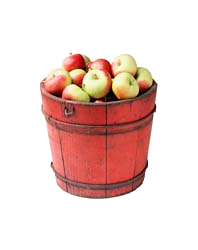
\includegraphics[height=2cm]{applebucket.png}&
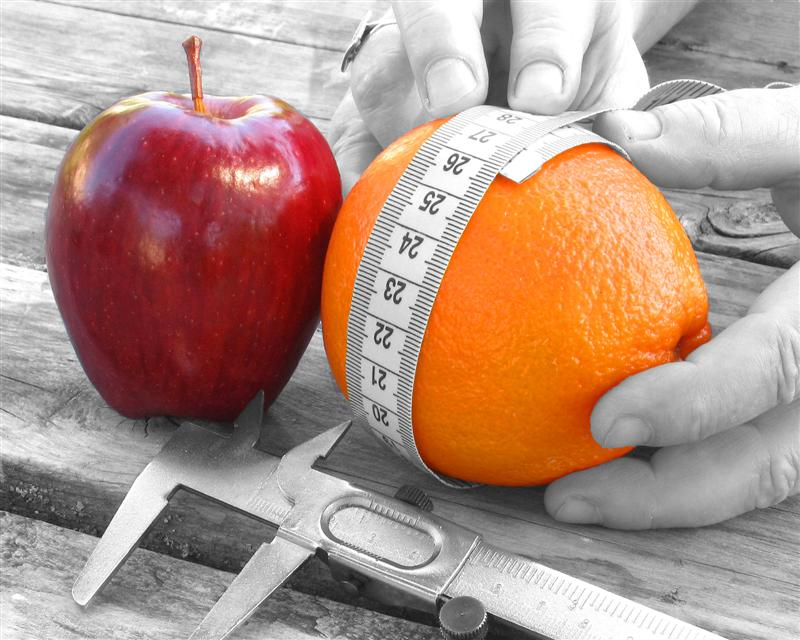
\includegraphics[height=2cm]{appleorange.jpg}&
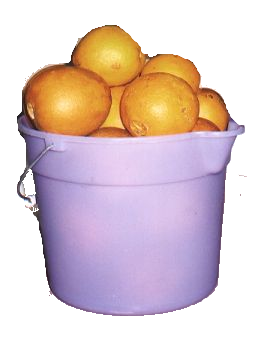
\includegraphics[height=2cm]{orangebucket.png}
\end{tabular}
\end{center}
\end{exampleblock}
\end{frame}

\begin{frame}
\frametitle{Sketched Digital Logic Symbols}
\begin{center}
\begin{tabular}{ccc}
``And''&``Or''&``Not''\\
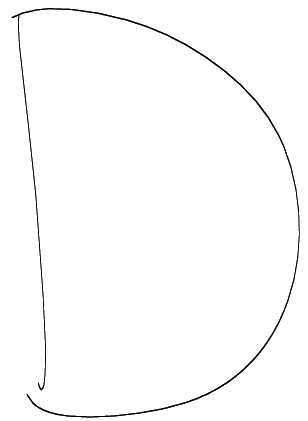
\includegraphics[height=3cm]{and.png}&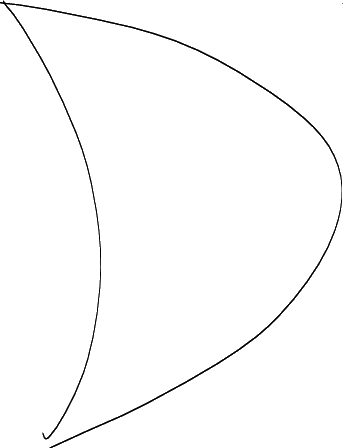
\includegraphics[height=3cm]{or.png}&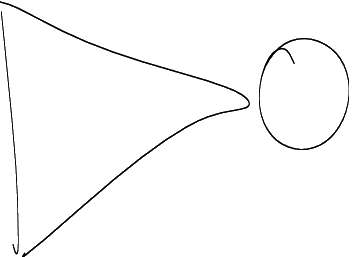
\includegraphics[height=3cm]{not.png}
\end{tabular}
\begin{tabular}{cc}
``Nor''&``Nand''\\
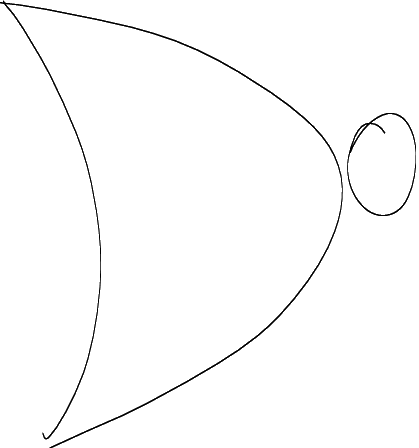
\includegraphics[height=3cm]{nor.png}&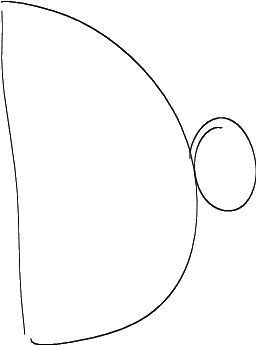
\includegraphics[height=3cm]{nand.png}
\end{tabular}
\end{center}
\end{frame}

\begin{frame}
\frametitle{Goal}
Develop a general sketched-symbol recognizer which returns a table of symbols and their associated probabilities.
For example, \\ \\
\begin{center}
\begin{tabular}{|l|ccccc|}
\hline
Symbol&And&Or&Not&Nor&Nand\\
\hline
Probability&0.20&0.73&0.01&0.05&0.01\\
\hline
\end{tabular}
\end{center}
\end{frame}

\begin{frame}
\frametitle{Problems with Raw Sketched-Symbol Data}
\begin{center}

\begin{itemize}
\item Overload of information\\ %need to extract essential info out, possibly infinite amount of points
\item Noise\\ %sampling rate of tablet
\item Hard to quantify\\ %useful information
\end{itemize}

\end{center}
\end{frame}

\begin{frame}
\frametitle{Potential Problems}
\begin{center}
\begin{tabular}{c}

\only<2>{Understroked Sketched-Symbol\\}
\includegraphics<2>[height=5cm]{andunder.png}

\only<3>{Overstroked Sketched-Symbol\\}
\includegraphics<3>[height=5cm]{andover.png}

\only<4>{Rotated Sketched-Symbol\\}
\includegraphics<4>[height=5cm]{andorient.png}

\only<5>{Ambiguous Sketched-Symbol\\}
\includegraphics<5>[height=5cm]{andor.png}

\end{tabular}
\end{center}
\end{frame}

\begin{frame}
\frametitle{Simplify our Data!}
\begin{center}
Working with raw sketch-symbol data presents many challenges. %as outlined above
One way to approach sketched-symbol recognition is to transform the data into a visual problem.
\end{center}
\end{frame}


\begin{frame}
\frametitle{Raw Sketched-Symbol to Image}
\begin{center}
\begin{tabular}{c}

\includegraphics<2>[height=4cm]{andthick.png}
\includegraphics<3>[height=4cm]{gridandthick.png}
\includegraphics<4>[height=4cm]{numbergrid.png}

\end{tabular}
\end{center}
\end{frame}

\begin{frame}
\frametitle{More Information from the Image}
\begin{center}
As we will see later, it is important that we can access a ``minimum-distance-to-pixel'' metric for every point $(x, y)$ in an image.
Thus, we will also need to create what is known as a distance transform.
\end{center}
\end{frame}

\begin{frame}
\frametitle{Image to Distance Transform}
\begin{center}
\begin{tabular}{cc}
Image&Distance Transform\\
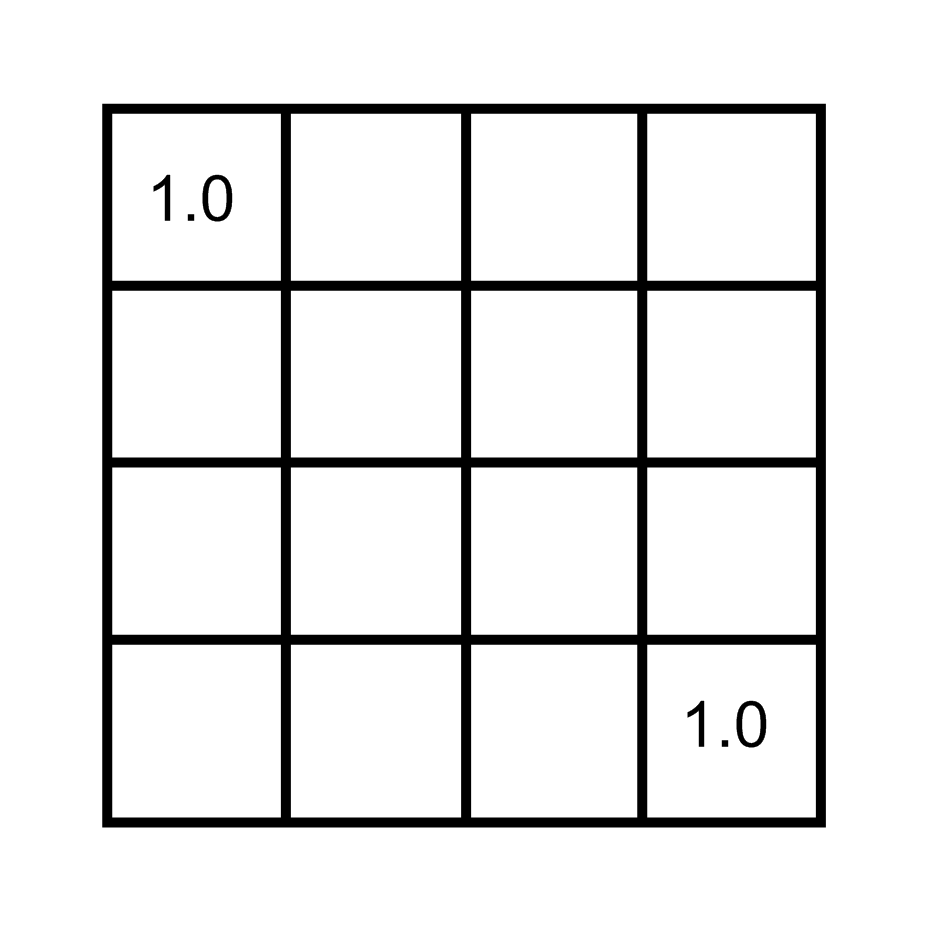
\includegraphics[height=4cm]{corners.png}&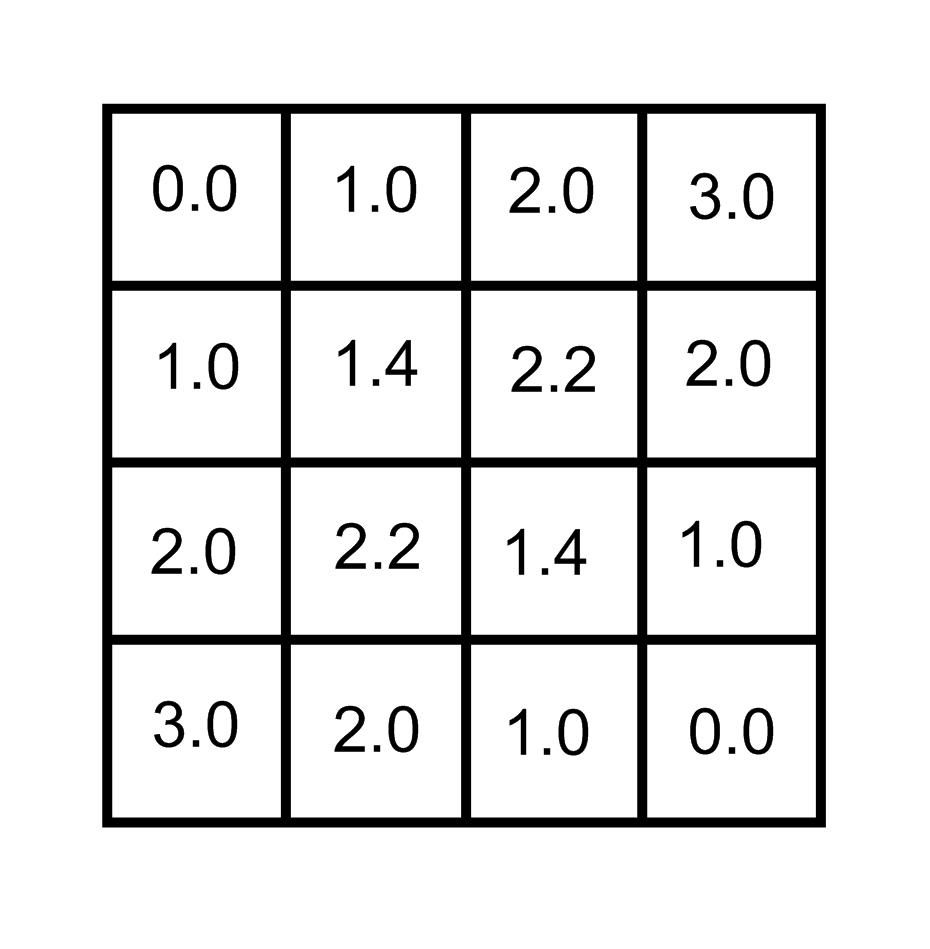
\includegraphics[height=4cm]{transform.png}
\end{tabular}
\end{center}
\end{frame}

\begin{frame}
\frametitle{Sketched-Symbols to an Average Image}
\begin{center}
\begin{tabular}{cccc}

\only<2>{&&&\multirow{6}{*}{\includegraphics<2>[height=5cm]{averagegrid.png}}\\}
\includegraphics<2>[height=1cm]{andthick.png}&\includegraphics<2>[height=1cm]{grid.png}\\
\includegraphics<2>[height=1cm]{and1.png}&\includegraphics<2>[height=1cm]{grid.png}\\
\includegraphics<2>[height=1cm]{and2.png}&\includegraphics<2>[height=1cm]{grid.png}&\includegraphics<2>[height=1cm]{rightarrow.png}\\
\includegraphics<2>[height=1cm]{and3.png}&\includegraphics<2>[height=1cm]{grid.png}\\
\includegraphics<2>[height=1cm]{and4.png}&\includegraphics<2>[height=1cm]{grid.png}\\

\end{tabular}
\end{center}
\end{frame}

\begin{frame}
\frametitle{Real Average Images}
\begin{center}
\begin{tabular}{cc}

\multicolumn{2}{c}{\only<1>{And}\only<2>{Or}\only<3>{Not}\only<4>{Nor}\only<5>{Nand}}\\
Average Image&Average Distance Transform\\
\includegraphics<1>[height=5cm]{andmain.png}\only<1>{&}\includegraphics<1>[height=5cm]{andmaintransform.png}
\includegraphics<2>[height=5cm]{ormain.png}\only<2>{&}\includegraphics<2>[height=5cm]{ormaintransform.png}
\includegraphics<3>[height=5cm]{notmain.png}\only<3>{&}\includegraphics<3>[height=5cm]{notmaintransform.png}
\includegraphics<4>[height=5cm]{normain.png}\only<4>{&}\includegraphics<4>[height=5cm]{normaintransform.png}
\includegraphics<5>[height=5cm]{nandmain.png}\only<5>{&}\includegraphics<5>[height=5cm]{nandmaintransform.png}

\end{tabular}
\end{center}
\end{frame}

\begin{frame}
\frametitle{Raw Sketched-Symbol to Polar Image}
\begin{center}
We also create average polar images, and average polar distance transforms.  
This helps our sketched-symbol recognizer deal with rotated sketched-symbols, as we will see later.
\end{center}
\end{frame}

\begin{frame}
\frametitle{Real Average Polar Images}
\begin{center}
\begin{tabular}{cc}
\multicolumn{2}{c}{\only<1>{And}\only<2>{Or}\only<3>{Not}\only<4>{Nor}\only<5>{Nand}}\\
Average Polar Image&Average Polar Distance Transform\\
\includegraphics<1>[height=5cm]{andpolar.png}\only<1>{&}\includegraphics<1>[height=5cm]{andpolartransform.png}
\includegraphics<2>[height=5cm]{orpolar.png}\only<2>{&}\includegraphics<2>[height=5cm]{orpolartransform.png}
\includegraphics<3>[height=5cm]{notpolar.png}\only<3>{&}\includegraphics<3>[height=5cm]{notpolartransform.png}
\includegraphics<4>[height=5cm]{norpolar.png}\only<4>{&}\includegraphics<4>[height=5cm]{norpolartransform.png}
\includegraphics<5>[height=5cm]{nandpolar.png}\only<5>{&}\includegraphics<5>[height=5cm]{nandpolartransform.png}
\end{tabular}
\end{center}
\end{frame}

\begin{frame}
\frametitle{Rotating a Sketched-Symbol to Match a Definition}
\begin{itemize}
\item<+-> Compute sketched-symbol's polar image around the weighted center.
\item<+-> Translate the polar image along the theta axis to match each the definition.
\item<+-> Rotate the initial sketched-symbol so that the orientation best matches that of the definiton.
\end{itemize}
\end{frame}

\begin{frame}
\frametitle{Illustrated Rotation}
\begin{center}
\begin{tabular}{ccccc}
&Sketched-Symbol&Image&Polar Image&And Definition\\
\only<2->{Original}&\includegraphics<2->[height=1.5cm]{rot.png}&\includegraphics<3->[height=1.5cm]{main8.png}&\includegraphics<3->[height=1.5cm]{polar8.png}&\multirow{1}{*}{
\includegraphics[height=1.5cm]{andpolar.png}}\\
\only<5->{Rotated}&\includegraphics<5->[height=1.5cm]{unrot.png}&\includegraphics<6->[height=1.5cm]{main8un.png}&\includegraphics<4->[height=1.5cm]{polar8un.png}
\end{tabular}
\end{center}
\end{frame}

\begin{frame}
\frametitle{Distance Metrics for Comparing Two Images}
\begin{itemize}[<+->]
\item Hausdorff Distance
\item Modified Hausdorff Distance
\item Tanimoto Coefficient
\item Yule Coefficient
\end{itemize}
\end{frame}

\begin{frame}
\frametitle{Hausdorff}
The Hausdorff distance between two binary images $A$ and $B$ is
$H(A, B) = \max(h(A, B), h(B, A))$,
where $h(A, B) = \max_{a \in A}(\min_{b \in B}||a - b||)$.
$h(A, B)$ is the directed Hausdorff distance.
Intuitively, every point in $A$ is at most a distance $h(A, B)$ away from some point in $B$.
\end{frame}

\begin{frame}
\frametitle{Modified Hausdorff}
$H_{mod}(A, B) = \max(h_{mod}(A, B), h_{mod}(B, A))$.
$h_{mod}(A, B) = \frac{1}{|A|}\sum_{a \in A}\min_{b \in B}||a - b||$, where $N_a$ is the number of points in $A$.
\end{frame}

\begin{frame}
\frametitle{Tanimoto}
$T_{sc}(A, B) = \alpha T(A, B) + (1 - \alpha)T^C(A, B)$,
where $T(A, B) = \frac{n_{ab}}{n_a + n_b - n_{ab}}$, $T^C(A, B) = \frac{n_{00}}{n_a + n_b - 2n_{ab} + n_{00}}$, and $\alpha = 0.75 - 0.25 (n_a + n_b) / (2N)$, where $n_{a}$ is the number of points in $A$, $n_{b}$ is the number of points in $B$, $n_{ab}$ is the number of overlapping points in $A$ and $B$, $n_{00}$ is the number of overlapping white-points in $A$ and $B$, and $N$ is the number of points in an image.
\end{frame}

\begin{frame}
\frametitle{Yule}
$Y(A, B) = \frac{n_{ab} n_{00} - (n_a - n_{ab})(n_b - n_{ab})}{n_{ab} n_{00} + (n_a - n_{ab})(n_b - n_{ab})}$
\end{frame}

\end{document}